\chapter{Mock-up}
A seguito delle problematiche e inesattezze mostrate nei capitoli precedenti, il pensare a una possibile soluzione � stata una logica conseguenza. L'elaborazione di modelli, grafici che consentano di risolvere gran parte dei problemi, o che riducano drasticamente la criticit�, prendono il nome di mock-up.\\
\'E da sottolineare come i mock-up siano un'astrazione e rappresentano comunque una visione soggettiva di come sarebbe possibile intervenire per migliorare l'usabilit� del sito web in esame; tale visione � influenzata dalle conoscenze del gruppo e dalle proprie esperienze pregresse.\\
Il primo punto da affrontare prima di concepire gli interventi veri e propri, � stato quello di decidere come affrontare i problemi:
\begin{itemize}
\item Come un singolo problema: ha il vantaggio di trattare modularmente ogni problema e ridurre cos� il rischio di generare nuovi problemi, durante la risoluzione. Lo svantaggio maggiore � rappresentato dal fatto che con questo metodo si rischia di generare ridondanza e di creare confusione per l'utente
\item Come collezioni di problemi: � il viceversa del caso precedente. Si riduce la ridondanza, si ha una visione pi� ampia dei problemi trovando delle soluzioni che possano andare bene per pi� problemi contemporaneamente, ma di conseguenza aumenta notevolemente il rischio di generare nuovi problemi
\end{itemize}
Nel nostro caso � stata scelta la seconda tecnica, in quanto trattandosi spesso di gruppi di pagine, era preferibile avere una visione d'insieme e trattare errori trasversali a pi� pagine, piuttosto che concentrarsi su errori di visibilit� limitata.\\
C'� anche un altro aspetto da mettere in evidenza, ma che spesso viene trascurato: il mock-up, inteso come strumento di presentazione, � solamente grafico, pertanto si potranno avere solamente degli screenshot di quello che potrebbe essere il risultato, nel caso la modifica riguardi il layout della pagina, ma come si � spesso notato, alcuni degli errori pi� gravi, riguardano l'aspetto implementativo; su tali errori si pu� solamente ragionare a livello teorico, ma l'implementazione di una soluzione non � fattibile in quanto mancano gli strumenti necessari alla realizzazione.\\ 
Verr� poi ricordato nelle varie sottosezioni, spesso vengono proposte soluzioni che per� andrebbero replicate su tutte o quasi le pagine del sistema. Spesso si tratta di link dai nomi non chiari, o la mancanza di un collegamento che semplificherebbe la vita all'utente.\\
\newline
Per poter ideare i mock-up � stato necessario lavorare su due livelli:
\begin{itemize}
\item Il primo livello � rappresentato dal lavoro direttamente sul codice HTML, e CSS, andando, tramite programmi apposta (es: firebug), a modificare il codice interpretato dal browser, potendo cos� ottenere risultati dall'effetto immediato e sopratutto senza modificare  lo stile della pagina. In tal modo i font utilizzati, i colori di sfondo e altri aspetti legati ai CSS sono rimasti invariati e si aveva un'idea immediata di cosa venisse mostrato all'utente
\item Il secondo livello � quello dei programmi di grafica (Gimp, Paint, Photoshop) utilizzati per i ritocchi pi� pesanti apportati alle pagine. Sono stati utilizzati pesantemente, quando la modifica del codice avrebbe richesto troppo tempo, in tal modo, tramite le opzione di ``taglia e incolla'' si � potuto disporre rapidamente gli elementi nella maniera che si � ritenuta pi� oppurtuna
\end{itemize}
\section{Mock-up home page sezione casa}
Prima di procedere con la presentazione dei mock-up ideati per questa sezione vi � un concetto che � bene ricordare: molti dei cambiamenti illustrati in questa sezione andrebbero riportati su tutte le pagine del sito web, poich� la mancanza o l'errore evidenziato � spesso replicato su tutte o quasi le pagine del sito web.\\
\begin{figure}[!h]
\centering
\includegraphics[scale=0.8]{figure/mock_up_home_page.eps}
\caption{Evidenziate in rosso il nuovo link all'Home page. \'E da replicare su tutte le pagine del sito web}
\label{fig:mock_up_non_loggato}
\end{figure}
\begin{figure}[!h]
\centering
\includegraphics[scale=0.8]{figure/mock_up_home_page2.eps}
\caption{Evidenziate in rosso il nuovo link all'Home page. Sono da replicare su tutte le pagine del sito web}
\label{fig:mock_up_non_loggato2}
\end{figure}
\begin{figure}[!h]
\centering
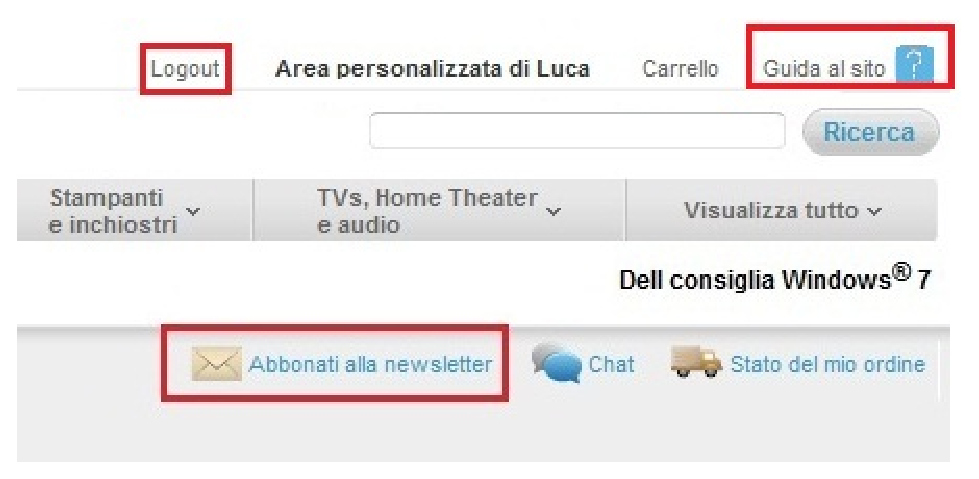
\includegraphics[scale=0.8]{figure/mock_up_home_page_loggato.eps}
\caption{Evidenziate in rosso le modifiche apportate alla home page quando l'utente � loggato}
\label{fig:mock_up_loggato}
\end{figure}
{\bf Descrizione:} non esiste un link chiaro per il ritorno all'home page, non c'� un link diretto che permetta a un nuovo utente di registrarsi e infine il link alla guida al sito � posto in fondo alla pagina, mischiato con altri link  e non viene in alcun modo evidenziato. Il link ``Registrazione e-mail'' non � esplicativa dell'effetto di tale registrazione.\\
{\bf Proposta di soluzione:} le soluzioni introdotte sono visibili nelle figure \ref{fig:mock_up_non_loggato} e \ref{fig:mock_up_non_loggato2}, e si possono riassumere come segue: accanto al marchio dell'azienda viene posto un link diretto all'home page. A destra vengono posizionati due link: ``Registrati'' e ``Guida al sito'', che forniscono all'utente quegli accelleratori che prima che mancavano; per completezza della pagina visualizzata quando l'utente non � ancora loggato (figura: \ref{fig:mock_up_non_loggato2}) di � anche pensato di modificare la scritta ``Sign In'', cambiandola con ``Accedi''. Nella parte sottostante il link ``Registrazione e-mail'' viene cambiato con ``Abbonati alla newsletter''.\\
La corrispettiva pagina che compare quando l'utente ha gi� effettuato l'accesso, mostra anzich� la dicitura ``Area personalizzata di Luca (L'utente corrente non � Luca?)'', mostra semplicemente ``Area personalizzata di Luca'' e posto a sinistra il link esplicito di logout.\\
\newline
All'interno di questa sezione abbiamo deciso d'inserire anche il mock-up del form di login, ed � stato modificato come in figura \ref{fig:form_login}.\\
{\bf Problema:} Il form del login � di per s� molto semplice e non ha avuto bisogno di un restyling degno di nota. Ci� che rappresenta il problema fondamentale, � il corretto funzionamento del sistema a fronte di due casi:
\begin{itemize}
\item Se si chiude la finestra di login durante la visualizzazione della progress barr, e successivamente si richiede un nuovo login il sitema � ancora in attesa della verifica dei dati inseriti precedentemente. Lo stato del sistema non cambia fintanto che l'utente non carica un'altra pagina o non effettua il refresh della pagina corrente
\item Dopo sei tentativi errati d'inserimento delle credenziali il sistema dovrebbe procedere alla disattivazione dell'account. Tuttavia inserendo le credenziali corrette, anche dopo sei tentativi errati l'account funziona correttamente
\end{itemize} 
{\bf Proposta di soluzione:} come detto in precedenza l'aspetto grafico della finestra non necessit� di grossi cambiamenti, e l'unico ad essere introdotto � composto dalla scritta che spiega il significato degli asterischi.\\ 
Diverso � l'intervento che si pu� pensare di apportare a livello implementativo:
\begin{itemize}
\item durante la fase di autenticazione, mentre vi � la progress bar, se la finestra viene chiusa erroneamente, il sistema dovrebbe poter in qualche modo ritornare allo stato precedente all'inserimento dei dati dell'account, invece ora il sistema rimane in una sorta di limbo, e se si richiede nuovamente al sistema di poter effettuare il login, il sistema risponde mostrando la finestra con la progress bar attiva, ma il sistema non si sblocca. 
\item Per quanto riguarda la disattivazine dell'account, abbiamo pensato che sia impossibile risalire a quale account l'utente volesse realmente accedere, pertanto poich� non pensabile disattivare account solo sulla base di supposizioni (lascerebbe troppo spazio d'azione a utenti hacker), si � pensato che si possa in qualche modo bloccare il computer che l'utente sta usando in quel momento: ad esempio impedire che effettui l'operazione di login per un determinato lasso di tempo, cos� da proteggere l'account da possibili attacchi.\\ 
\end{itemize}
\begin{figure}[!h]
\centering
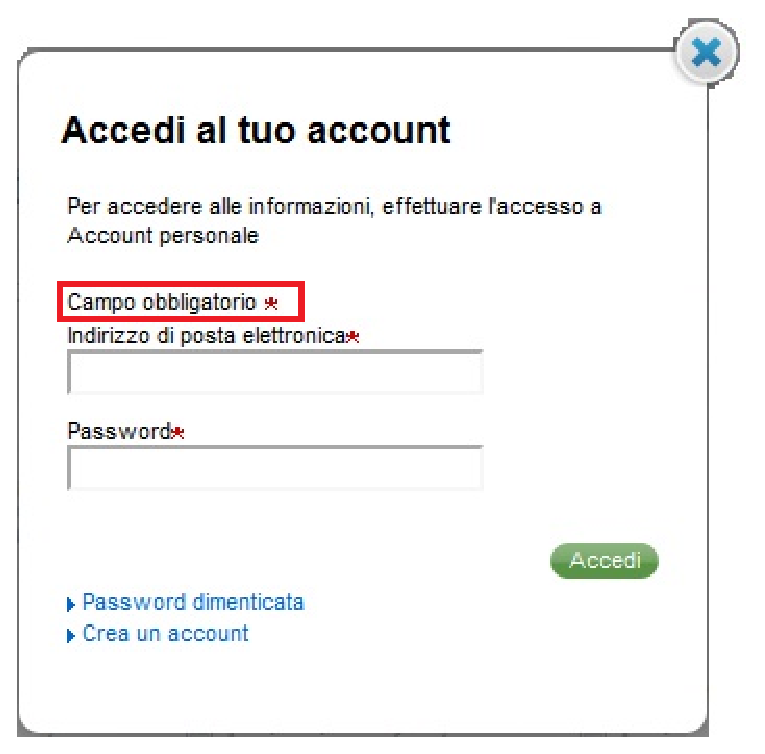
\includegraphics[scale=0.65]{figure/mock_up_fom_login.eps}
\caption{Evidenziate in rosso le modifiche apportate alla home page quando l'utente � loggato}
\label{fig:form_login}
\end{figure}

{\bf Descrizione}: all'interno della pagina relativa ai dati personali dell'utente non esiste un link che rimandi alla pagina in cui l'utente pu� cancellare il proprio account. Ci� rimane estremamente vincolante poich� un utente dovrebbe avere la libert� di potersi disiscriversi in ogni momento.
{\bf Proposta di soluzione}: all'interno della pagina contenente i dati personali viene aggiunta una voce al men� di sinistra riportante la voce ``cancellazione account''. In tal modo si pu� accedere a una sezione, che verr� aperta sulla destra, rispetto al men�, in cui l'utente potr� disiscriversi. Dal punto di vista implementativo, si � pensato di far comparire una finestra a popup, che per chiedere la conferma e come vincolo di sicurezza, richiede la password dell'account(figura \ref{fig:mockup_cancellazione_account}).

\begin{figure}[!h]
\centering
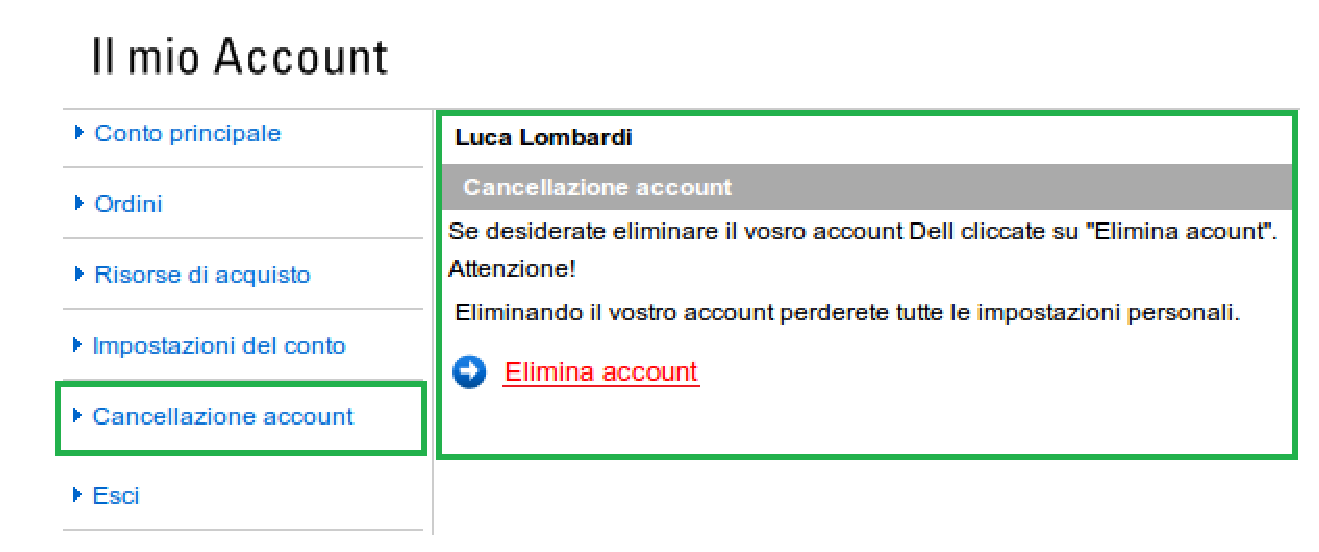
\includegraphics[scale=0.7]{figure/mock_up_cancellazione.eps}
\caption{In verde sono evidenziate le parti aggiunte che consentono all'utente di disiscirversi}
\label{fig:mockup_cancellazione_account}
\end{figure}

{\bf Descrizione}: come detto nella sezione dedicata ai problemi di usabilit�, se nel momento in cui il sistema sta verificando le credenziali, l'utente chiude la finestra di dialogo, il sitema rimane in uno stato ibrido in cui l'utente non pu� effettuare un nuovo login e il sistema non riconosce ancora l'utente.\\
{\bf Proposte di soluzione}: per ovviare a tale problema si � pensato di modificare la pagina che compare alla chiusura della finestra di dialogo, come mostrato in figure \ref{fig:mock_up_login_reindirizzo}. In tal modo si d� l'opportunit� all'utente di forzare il sistema ad uscire dallo stato ibrido nel quale � caduto, tramite l'intervento guidato dell'utente.\\

\begin{figure}[!h]
\centering
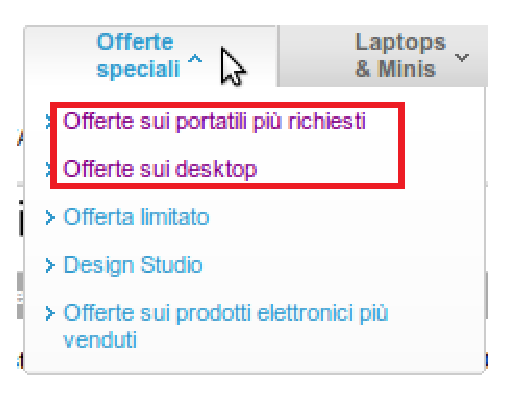
\includegraphics[scale=0.6]{figure/mock_up_link_usati.eps}
\caption{Riquadrati in rosso la modfica del colo dei link gi� selezionati dall'utente}
\label{fig:mock_up_link_usati}
\end{figure}

{\bf Descrizione}: come segnalato in precedenza, il sistema in nessuna sua parte, d� mai all'utente un riscontro sui link gi� usati, all'interno di una stessa sessione di lavoro.\\
{\bf Proposte di soluzione}: come riportato in figura \ref{fig:mock_up_link_usati} si pu� notare come i link selezionati almeno una volta siano colorati in modo diverso, dando all'utente un aiuto qualora cerchi una pagina visitata in precedenza e l'operatore di UNDO del browser non gli possa essere d'aiuto.

\begin{figure}[!h]
\centering
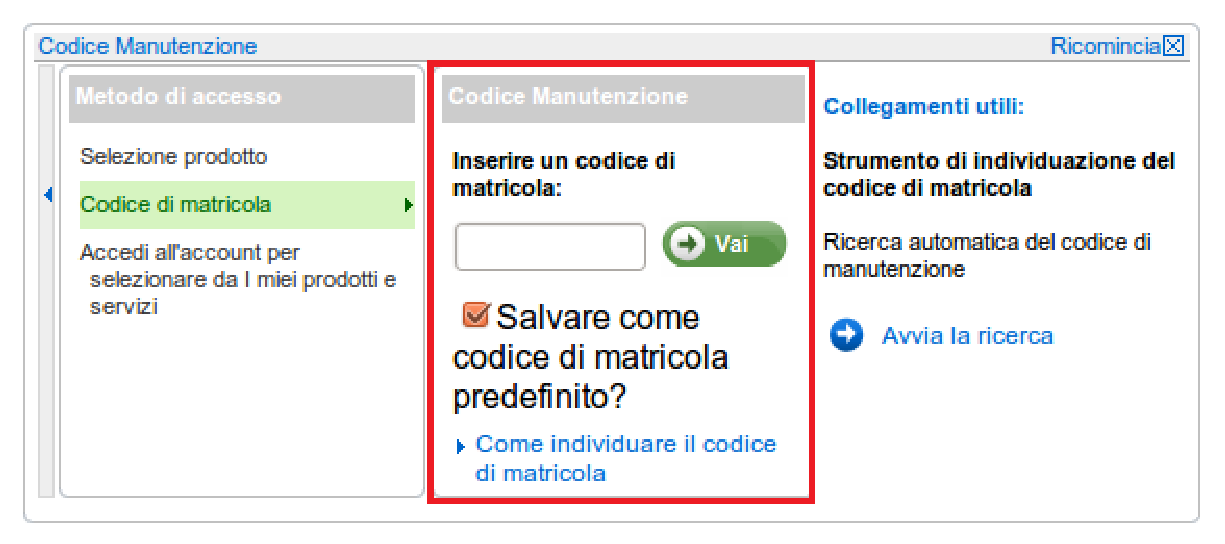
\includegraphics[scale=0.75]{figure/mock_up_manutenzione.eps}
\caption{il men� viene espanso leggermente per evitare la scroll bar, come invece era fatto nella versione originale (figura:\ref{fig:manutenzione})}
\label{fig:mock_up_manutenzione}
\end{figure}

{\bf Descrizione}: dalla figura \ref{fig:manutenzione} di nota che l'area dedicata al ``Codice Manutenzione'', � estramente ridotta e si deve ricorrere a una scroll bar per consentire all'utente di visualizzare tutto il contenuto: ci� risulta estremamente scomodo, considerato che il resto della pagina � inutilizzato.\\
{\bf Proposte di soluzioni}: viene ampliata l'intera area, fino a che la scroll bar non scompare, in tal modo l'utente pu� accedere a tutte le informazioni in modo diretto senza intralci.


\begin{figure}[!h]
\centering
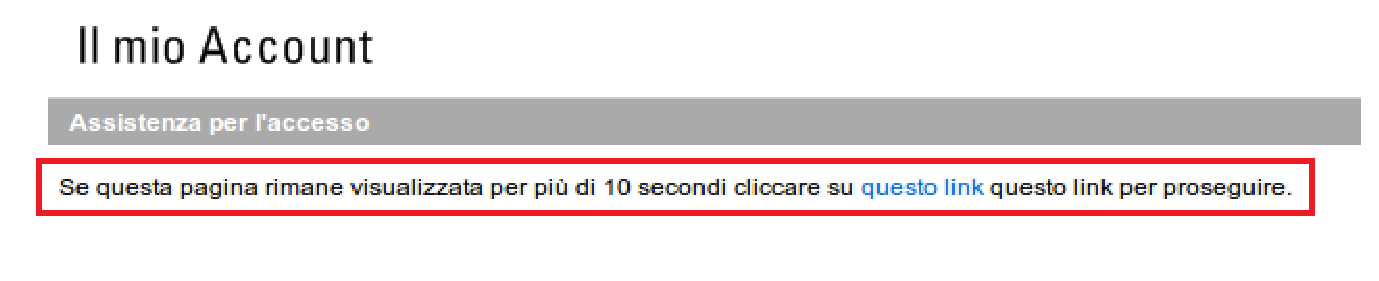
\includegraphics[scale=0.6]{figure/mock_up_login_reindirizzo.eps}
\caption{Nel caso il form del login non reindirizzi automaticamente, viene data la possibilit� all'utente di agire manualmente}
\label{fig:mock_up_login_reindirizzo}
\end{figure}
{\bf Descrizione}: nella figura \ref{fig:mock_up_riepilogo} sono evidenziate le piccole modifiche apportate alla pagina di configurazione del propriro sistema Dell. Come anticipato nella sezione relativa ai problemi di usabilit�, la pagina relativa alla scelta per la copertura sui danni accidentali, non ha alcun riferimento alle condizioni contrattuali, ma solo vaghe spiegazioni dal carattere pubblicitario. Inoltre la finestra di riepilogo delle componenti scelte per la personalizzazione � molto ristretta, costringendo l'utente a un continuo uso dello scroll per scorrere tale riassunto.\\
{\bf Proposta di soluzione}: viene aggiunto un link alla documentazione per gli esatti termini contrattuali dell'estensione di garanzia proposta. Inoltre come si pu� notare a destra, la finestra di riepilogo dei componenti selezionati dall'utente viene espansa in modo da mostrare pi� componenti contemporaneamente.
\begin{figure}[!h]
\centering
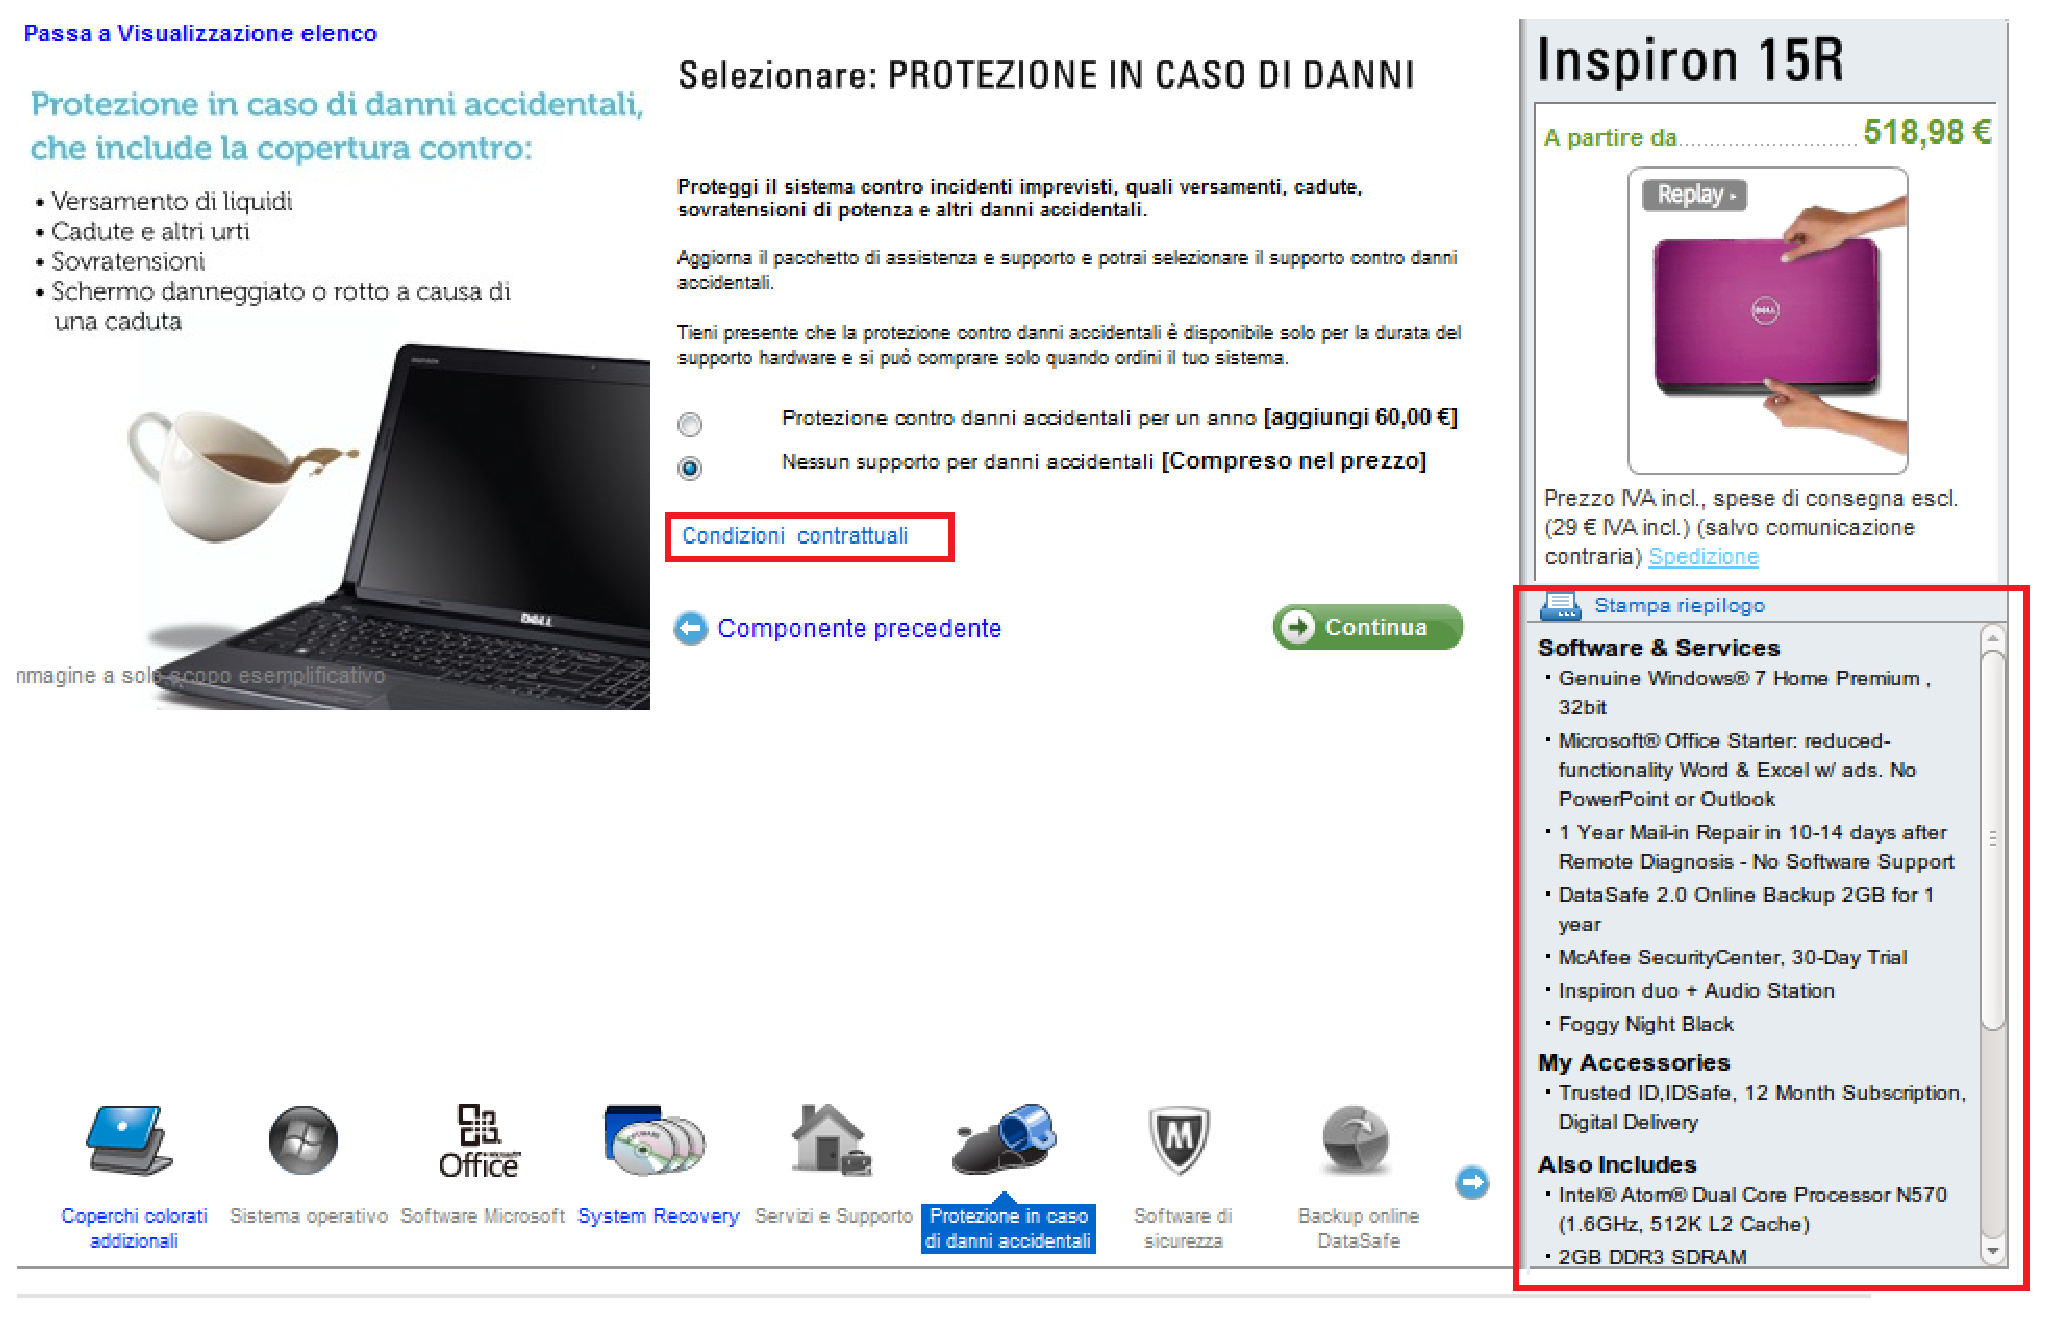
\includegraphics[scale=0.7,angle=90]{figure/mock_up_riepilogo.eps}
\caption{Mock-up sulla pagina di configurazione del computer}
\label{fig:mock_up_riepilogo}
\end{figure}

Come anticipato nella sezione relativa ai problemi di usabilit�, un problema no un certo rilievo � quello del sovraffollamento dell'home page delle due sezioni ``Acquista'' e ``Supporto'' che rendono difficoltosa la navigazione. In questa parte analizzeremo le due soluzioni proposte, motivando le scelte effettuate.
\begin{itemize}
\item {\bf Sezione Acquisti}: per prima � stata analizzata la home page della sezione degli acquisti. Come si pu� notare dalle figura mostrata nella sezione relativa ai problemi di usabilit�, alla figura: \ref{fig:schermata_incasinata}, la pagina mostrata all'utente � densa di banner pubbblicitari, che creano confusione, e duplicano tutti i link. Dal punto di vista del marketing, sicuramente � utile avere una pagina formattata in tale maniera, poich� come detto, il sito ha anche lo scopo di essere una vetrina d'esposizione per i prodotti dell'azienda, tuttavia dal punto di vista della navigabilit� non � ottimale.\\

{\bf Proposte di soluzione}: per ovviare a tali problemi si � pensato a un netto snellimento dei contenuti, che tuttavia non percludono la possibilit� di aggiungere della pubblicit�, ma � la pagina risulta decisamente pi� facile da navigare e le informazioni utili sono al centro dell'attenzione, e non mescolate alla pubblicit� come acadeva prima.\\
Nella figura \ref{fig:mockup_sez_acquisti_pagina_intera} si pu� vedere come si � pensato di riorganizzare il tutto:
\begin{itemize}
\item Innanzitutto spariscono tutte le immagini pubblicitarie che potranno essere poste ai lati del corpo centrale della pagina
\item Di tutte e sei le sezioni pre-esistenti (vedere figura:\ref{fig:schermata_incasinata}) vengono mantenute solamente quattro categorie che racchiudono tutti i prodotti: ``Notebook \& Mini'', ``Desktop e All-in-One'', ``Monitor'', ``Elettronica ed Accessori''. Tramite queste si accede alle sottosezioni. Si � ritenuto utile porre al di sotto di ogni immagine una serie di qualche link, come accelleratori per poter incentivare la visita delle pagine relative a dei prodotti sulla quale l'azienda vuole maggiormente puntare come vendita, ma in ogni caso tali link non costituiscono la parte preponderante della pagina e non sono d'intralcio nella navigazione
\item Al di sotto di questa sezione vengono proposti due link in chiara evidenza, nel caso l'utente necessitasse o volesse richiedere assistenta per l'acquisto di un qualsiasi prodotto. I due link scelti sono quelli dell'assistenza tramite una chat oppure assistenza telefonica. \'E stato ritenuto sufficiente questo tipo di aiuto, poich� come segnalato, le finestre a pop-up o altri tipi di avvisi per richiedere assistenza spesso erano pi� dannosi che altro (Es: il link per la chat che navigava all'interno della pagina)
\end{itemize}

\begin{figure}[!h]
\centering
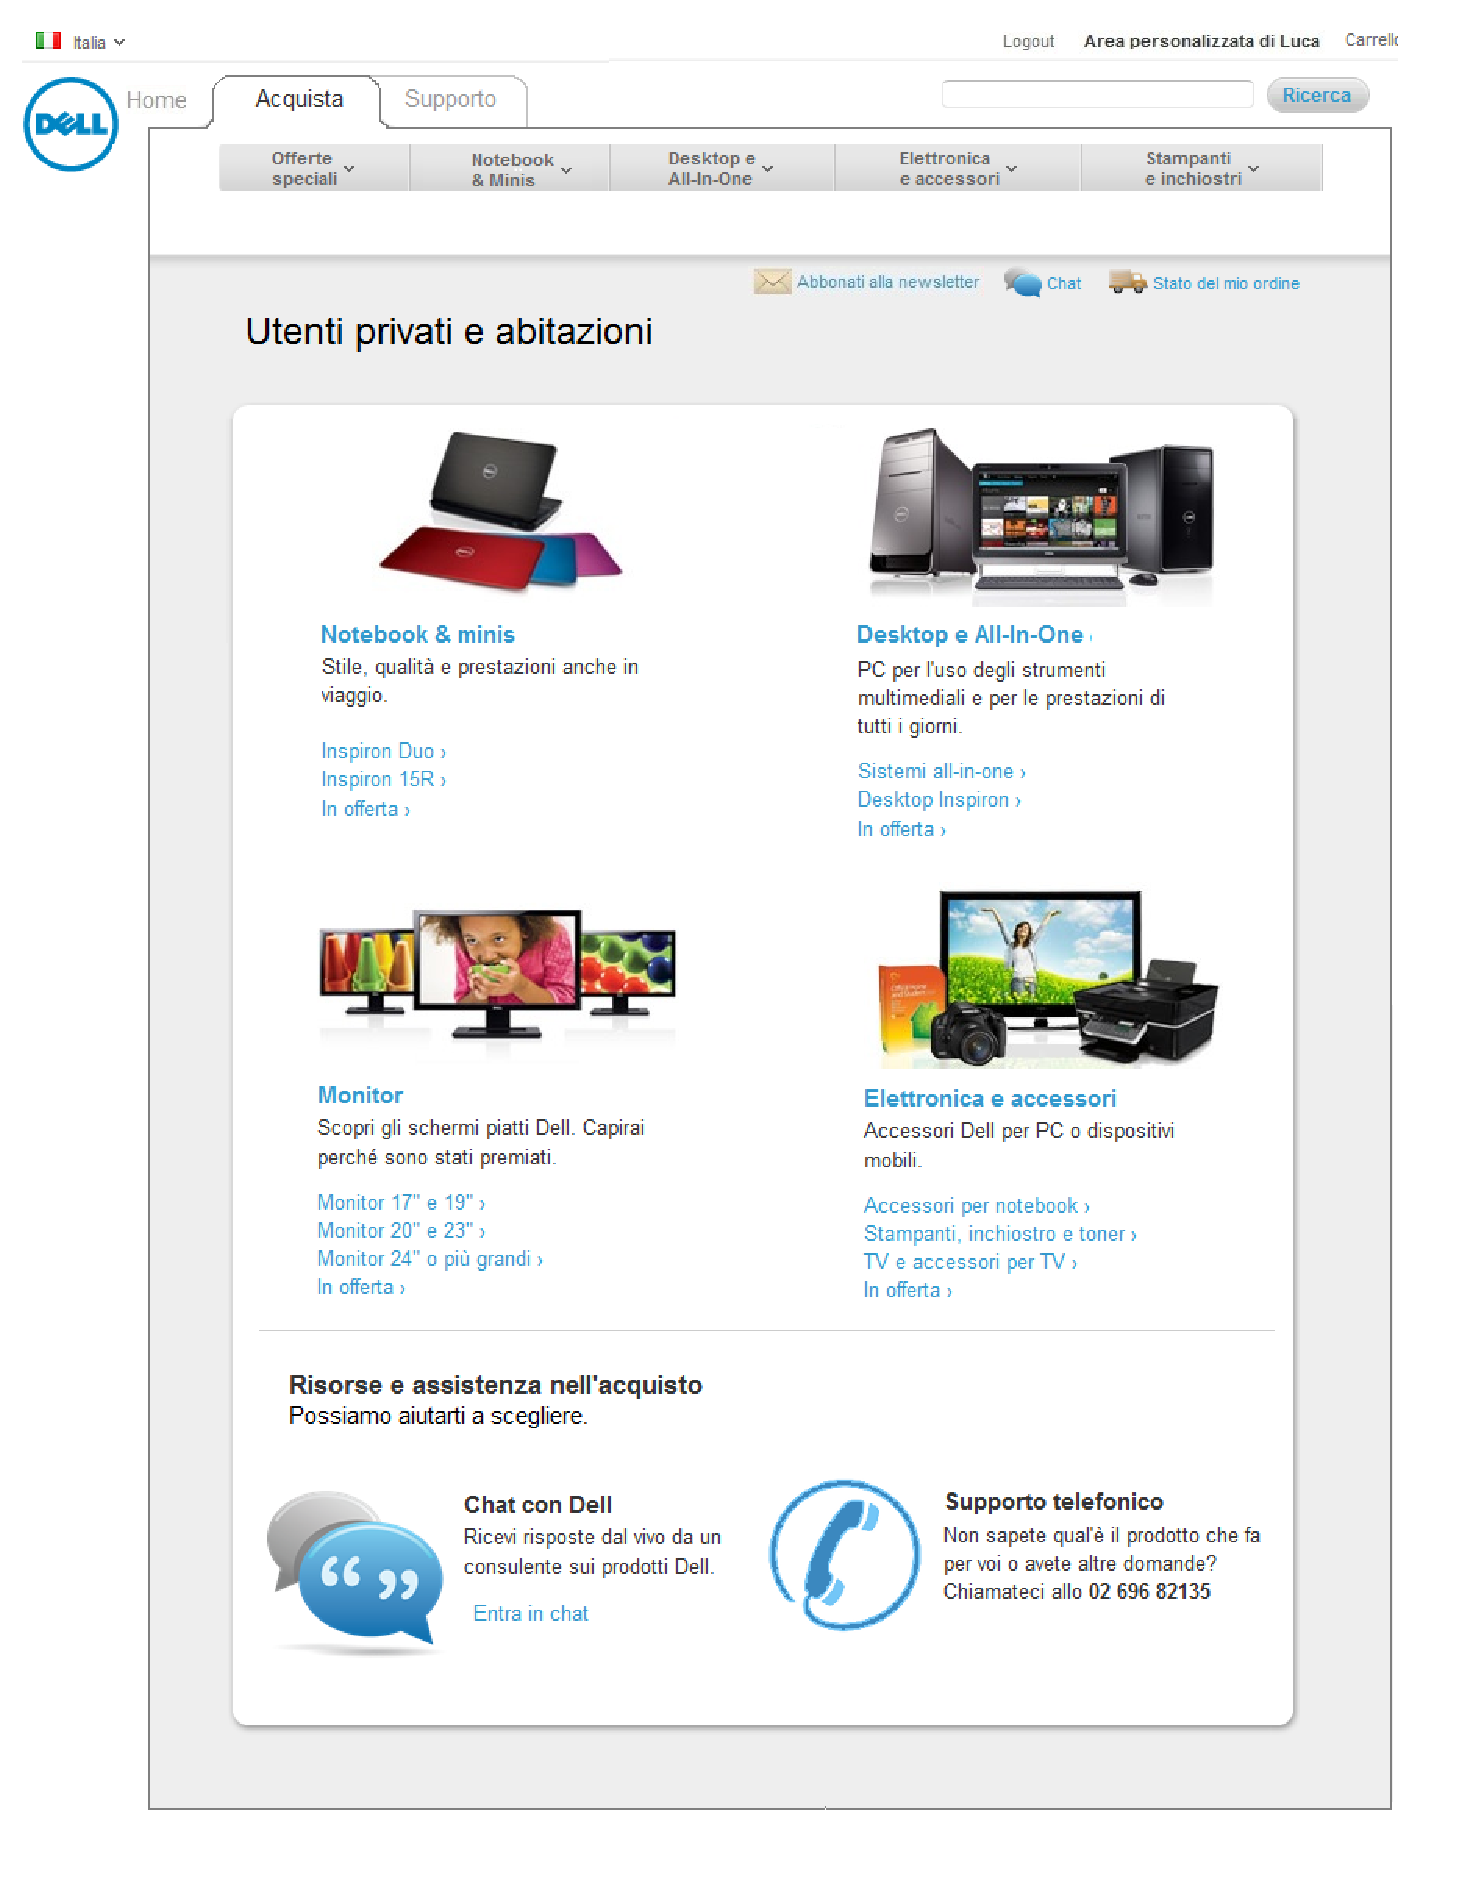
\includegraphics[scale=0.52]{figure/mockup_sez_acquisti_pagina_intera.eps}
\caption{Mock-up della sezione degli acquisti}
\label{fig:mockup_sez_acquisti_pagina_intera}
\end{figure}

\item{\bf Descrizione}: la sezione di supporto, seppur in forma minore, soffre anch'essa del problema della home page della sezione acquisti, ossia di sovraffollamento di link spesso ripetuti che creano solamente confusione per l'utente meno esperto. In questa sezione non si hanno banner pubblicitari, ma la pagine risulta essere densa di scritte e le immagini spesso sono splicative, ma racchiudono solamente macro gruppi di link, che risultano essere lunghi da leggere.
{\bf Proposte di soluzione}: per migliorare la pagina sono state introdotte radicali modifiche al layout:
\begin{itemize}
\item I quattro gruppi principali di icone poste a centro pagina, sono stati unite ai sei che si trovano poco pi� sotto, all'interno della parte ``Altri strumenti di supporto''. In tal modo si sono ottenuti sette macro insiemi che racchiudono e suddividono in categorie tutte le tipologie di problemi che potrebbe avere l'utente. Tali categorie sono:
\begin{itemize}
\item Driver e Hardware: sezione dedicata ai driver, aggiornamenti e richiesta di assistenza per  l'hardware del computer. Da tale sezione di pu� accedere alla sezione di download di aggiornamenti per firmware e altro software strttamente legato al funzionamento dei componenti fisici del computer
\item Guide e Tutorial: sezione dedicata alla documentazione per poter consentire all'utente di imparare da manuali e trovare risposte alla domande pi� frequenti
\item Supporto per Windows: sezione che riguarda tutti i sistemi Microsoft che sono venduti sulle macchine Dell. All'interno si accede a una pagina che permette all'utente di scegliere fra i vari sistemi operativi, trovare risposte che riguardano il buon funzionamento del sistema operativo
\item Stato dell'ordine e supporto: sezione rivolta a chi necessita di avere risposte e assistenza per effettuare correttamente un ordine, avere notizie riguardate lo stato si un ordine gi� effettuato
\item Sicurezza e virus: sezione dedicata alla sicurezza del sistema Dell acquistato
\item Connettivit� e reti: sezione dedicata alla configurazione e gestione di una rete domestica, sia calbata che wireless
\item Stampanti e altre periferiche: sezione dedicata all'installazione e configurazione in una periferica collegata poi a un sistema Dell. In tale sezione si trova anche supporto per le periferiche di marchio Dell
\end{itemize}
\item Al di sotto delle 7 esplicate in precedenza, la pagina mostra altri quattro gruppi che non potevano essere accorpati a quelli precedenti, e non hanno la stessa importanza:
\begin{itemize}
\item Forum Dell: link dedicato all'accesso alla community per avere assistenza da altri utenti
\item Informazioni sulla garanzia: link che permette di accedere alla visione del contratto di garanzia che l'utente stipula al momento dell'acquisto di un prodotto Dell
\item Cronologia e stato di supporto: qualora la richiesta di assistenza non fosse immediatamente soddisfatta, in questa sezione l'utente pu� avere informazioni e aggiornamenti sulla propria domanda di supporto
\item Strumenti e applicazioni: sezione dedicata a come trovare i vari codici, e diciture dei compoenti hardware e software che sono spesso richiesti dall'assistenza
\end{itemize}
\item A fianco del corpo centrale, a sinistra � riproposta una colonna di link, che a dispetto della versione precedente (figura: \ref{fig:supporto_senza_modifiche}), ha molti meno link. Nella nuova versione infatti sono stati riportati solamente:
\begin{itemize}
\item un link all'home page della sezione di supporto;
\item una serie di contatti diretti con gli operatori specializzati (vendita, ordine, tecnici)
\item una lista composta da otto link, che riportano le otto domande pi� frequenti poste nell'ultimo periodo. Tale lista � variabile, in quanto le domande pi� cercate cambieranno nel tempo, ma � utile mostrarle all'utente per consentire ad utenti pi� esperti di avere degli accelleratori adeguati
\end{itemize}
\end{itemize}
\end{itemize}
\begin{figure}[t]
\centering
\includegraphics[scale=0.5]{figure/supporto_senza_modifiche.eps}
\caption{Home page della sezione di supporto prima delle modifiche}
\label{fig:supporto_senza_modifiche}
\end{figure}

\begin{figure}[!h]
\centering
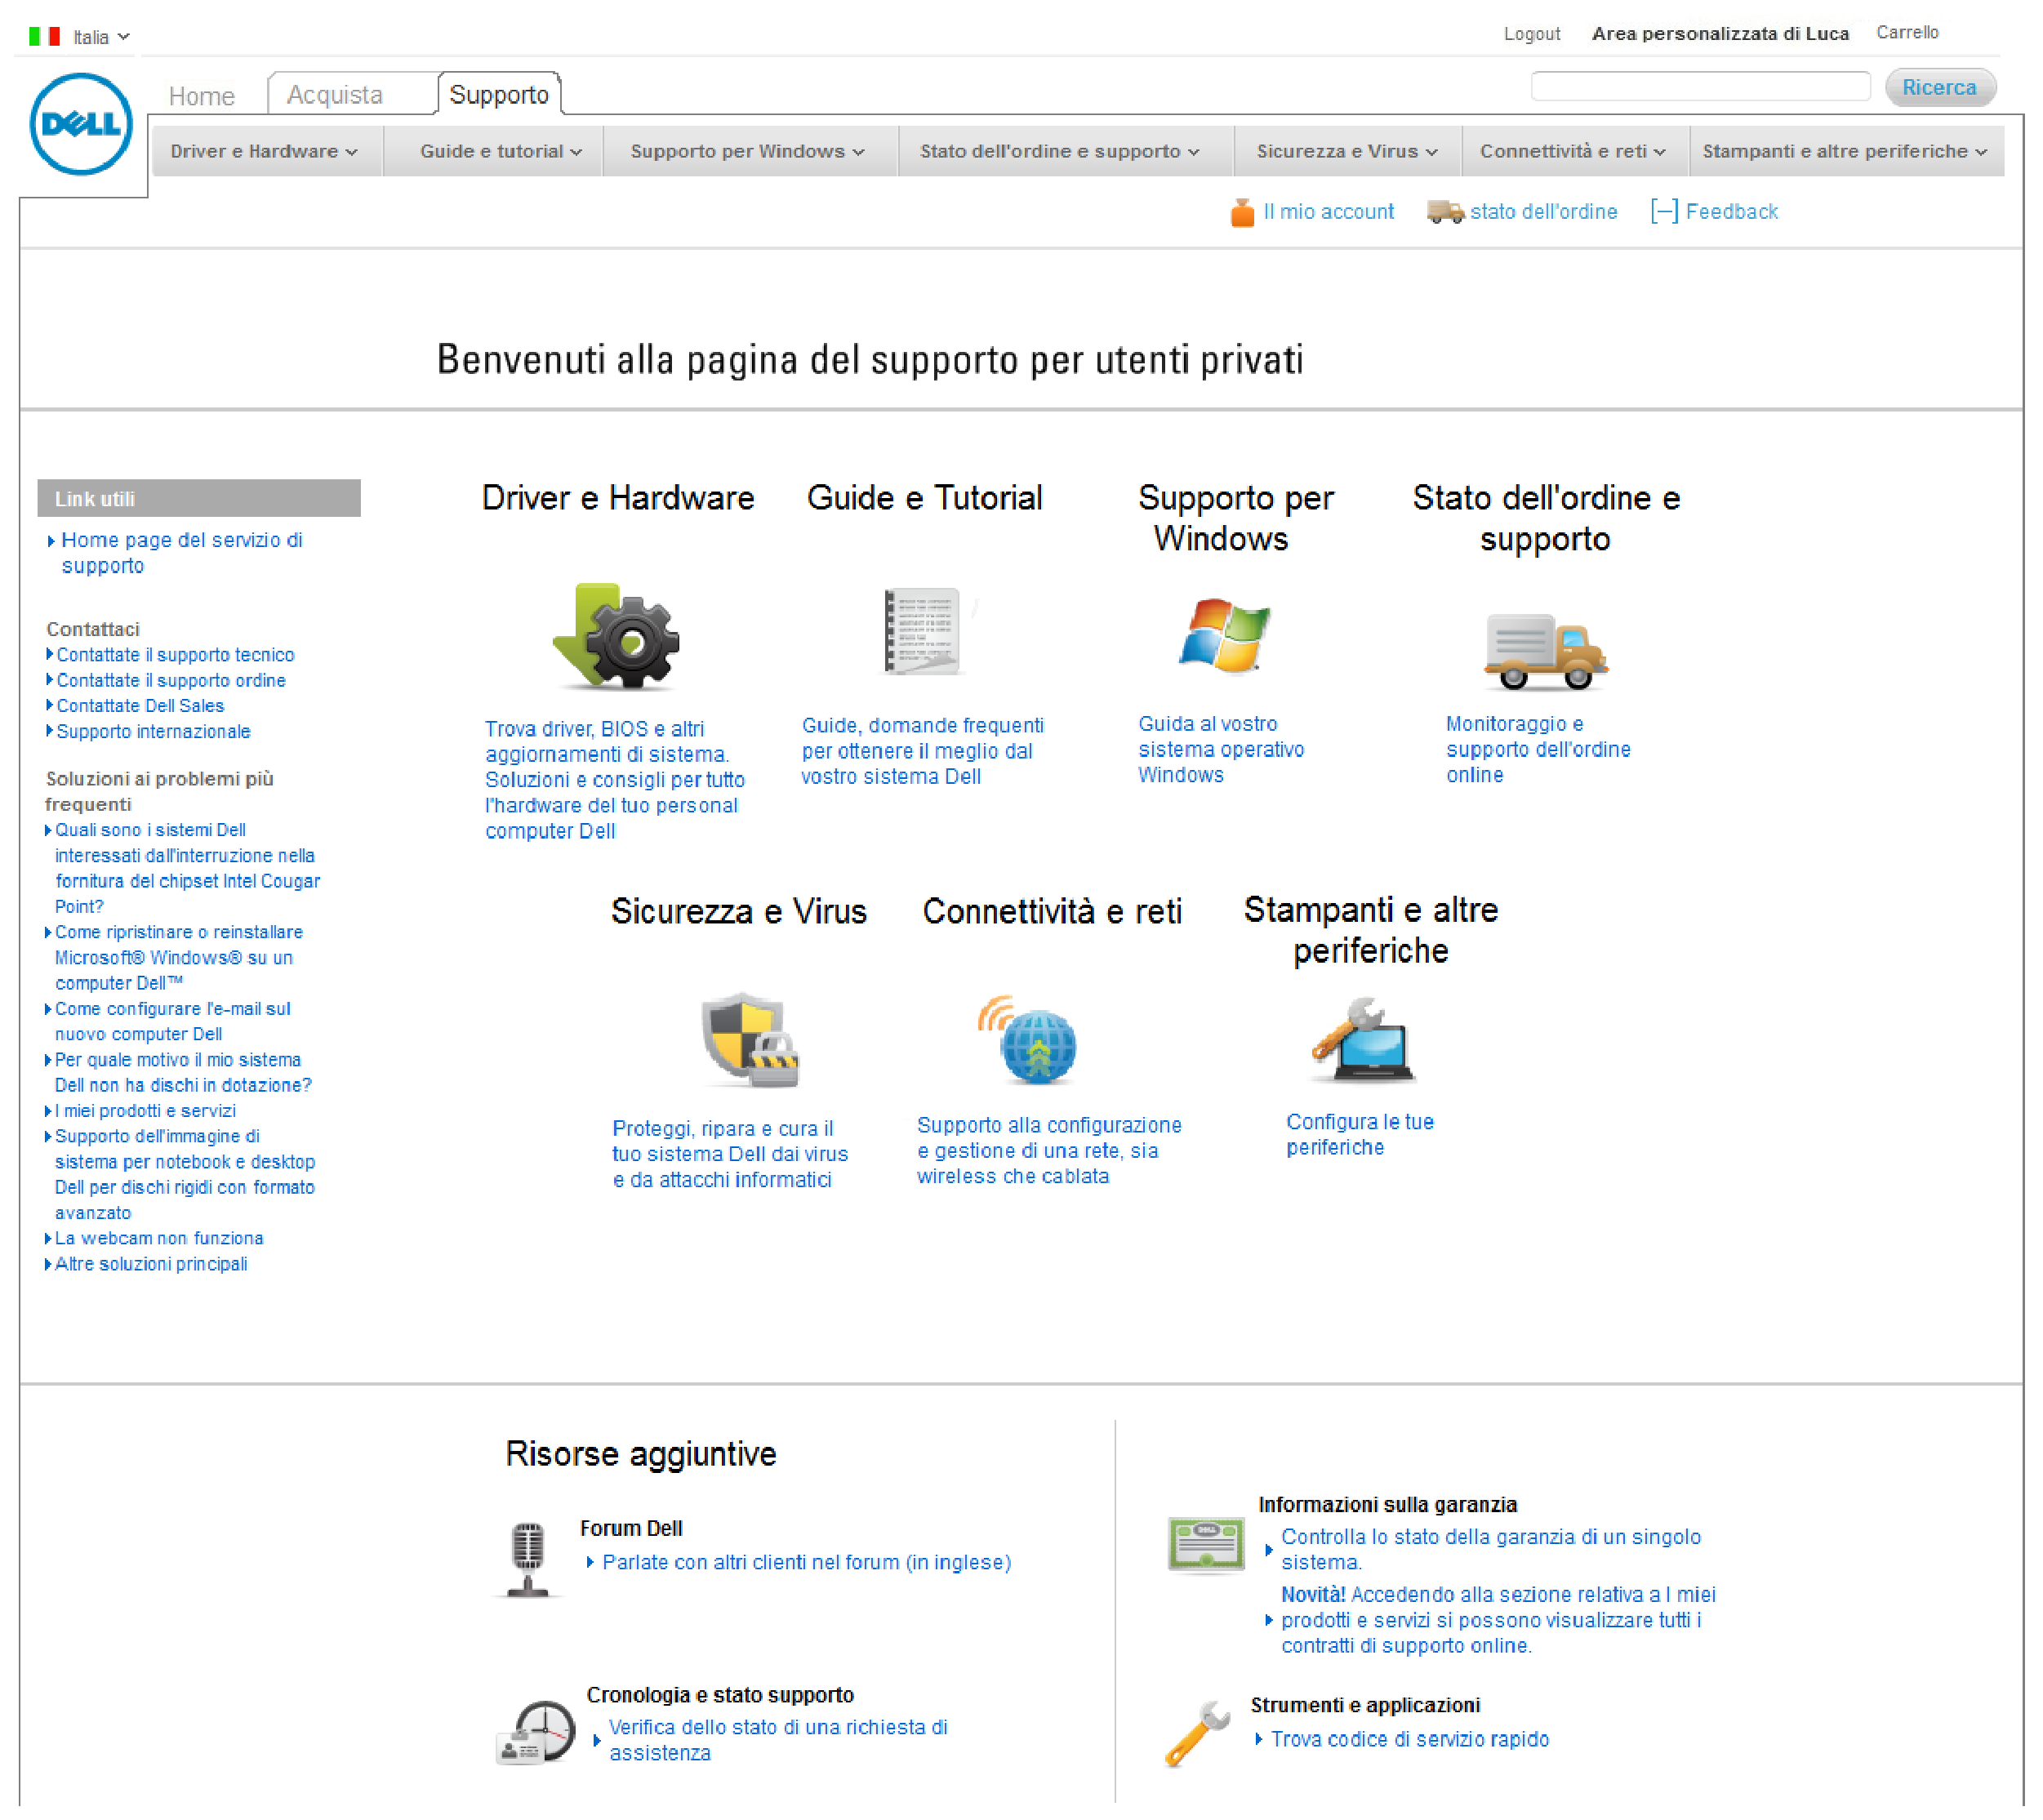
\includegraphics[angle=90,scale=0.45]{figure/mock_up_home_supporto.eps}
\caption{Mock-up della home page della sezione di supporto}
\label{fig:mock_up_home_supporto}
\end{figure}

